\documentclass[bibtotocnumbered, headsepline,normalheadings,12pt,polish]{scrreprt}
\usepackage[T1]{fontenc}
\usepackage[utf8]{inputenc}
\usepackage{geometry}
\geometry{tmargin=25mm,bmargin=25mm,lmargin=30mm,rmargin=30mm}
\usepackage{babel}
\setlength\parindent{0pt}
\usepackage{graphics}
\usepackage{floatflt}
\usepackage{scrpage}
\usepackage{alltt}
\usepackage{pdfpages}
\usepackage{hyperref}
\usepackage{moreverb}
\usepackage{enumerate}

\pagestyle{headings}
\begin{document}
\title{\textbf{Implementacja algorytmu genetycznego.\\Prototyp 2\\(z Circle Packing)}\\
\small{Algorytmy i Struktury Danych\\ Wydział Elektryczny, Politechnika Warszawska}}
\author{Tomasz Sobutka \and Artur Skonecki \and Prowadzący: Bartosz Chaber}
\date{Wygenerowano: \today}
\maketitle

%\tableofcontents

%\chapter{Wstęp}
%\section{Algorytmy genetyczne }
%Służą do wyznaczenia najlepszego rozwiązania złożonego problemu ze względu na przyjęte kryterium(wskaźnik) jakości. Nazwa nie przypadkowo kojarzy się z biologią, gdyż autor tej metody inspirował się teorią Darwina. Algorytmy te chechują się tym, że dobrze znajdują naraz więcej niż jedno minimum lokalne. Są stosowane wtedy gdy niemożliwe jest przejrzenie całego zbioru rozwiązań, ale łatwo można dobrać kryteria jakości rozwiązania. 
% 
%\section{ Przebieg algorytmu}
%\begin{enumerate}
%    \item Tworzona jest początkowa populacja osobników
%    \item Dokonywana jest selekcja osobników. Te najlepsze będą poddane procesowi reprodukcji.
%    \item Przeprowadzane są operacje krzyżowania i mutacji na wyselekcjonowanych osobnikach.
%    \item Sprawdzane jest najlepsze rozwiązanie . Jeśli jest ono wystarczająco dobre algorytm kończy działanie. 
%    \item Na kolejnym pokoleniu dokonywana jest selekcja (żeby utrzymać stałą liczbę osobników). Algorytm wraca do punktu 3.
%\end{enumerate}
%
%\section{Chromosom}
%Jest to struktura danych, określająca danego osobnika. Innymi słowy są to cechy, które umożliwiają znalezienie rozwiązania problemu. Chromosom składa się z pojedynczych genów. Zestaw genów, który charakteryzuje konkretnego osobnika to genotyp.
%
%\section{ Populacja początkowa}
%Stworzenie początkowej populacji może być wykonane na różne sposoby. Można wylosować całą populację. Można zaprojektować kilka rozwiązań odwołując się do swojej wiedzy o problemie a resztę osobników dobrać losowo. Można również posłużyć się już wcześniej wyprodukowanymi osobnikami z poprzednich przebiegów algorytmu. Ważny jest też odpowiedni dobór liczebności. Zbyt duża populacja może powodować duże zużycie zasobów sprzętowych, zbyt mała słabą jakość wyników.
%
%\section{ Funkcja przystosowania}
% Funkcja ta ocenia jakośc rozwiązania na podstawie wartości cech. Jest ona obliczana dla każdego osobnika i sprawdzana jest przydatność osobnika w populacji. Na podstawie wartości tej funkcji przeprowadzana jest selekcja.
%
% \section{ Metody selekcji}
%\begin{itemize}
%    \item Koło ruletki – Im lepszy jest dany osobnik tym ma większą szansę na zostanie w populacji. Ten algorytm nie sprawdza sie zbyt dobrze ze względu na możliwą eliminację najlepszych rozwiązań, z drugiej strony mamy wtedy większą rożnorodność osobników.
%    \item Metoda rankingowa – Ustawiamy wszystkie osobniki na liście według wartości funkcji dostosowania i bierzemy najlepsze osobniki. Metoda ta ma jednak wadę w postaci przedwczesnej zbieżności do pewnej grupy rozwiązań. 
%    \item Metoda turniejowa – Tutaj dzielimy populację losowo na małe grupy, po czym z każdej grupy wybieramy dwa najlepsze osobniki, które będą stanowić parę rodziców przyszłego potomstwa. Ta metoda eliminuje częściowo wady wyżej wymienionych metod.
%\end{itemize}
%\section{ Krzyżowanie}
%Polega na łączeniu dwóch genotypów w jeden. Może być zrealizowane na różne sposoby. Na przykład część genotypu(niekoniecznie połowa) wzięta z pierwszego genotypu, reszta z drugiego. Można też losować przy każdym genie, z którego genotypu będzie wzięty dany gen.
%
%\section{ Mutacja}
%Jest to metoda, która przeprowadza niewielkie zmiany w genotypie po to by różnicować rozwiązania. Jej prawdopodobieństo jest na tyle małe by nie wprowadzić efektu odwrotnego.
%
%\section{ Zastosowania algorytmów genetycznych  }
%Rozwiązywanie problemów NP-trudnych. Są to zadania, gdzie nie jest dobrze poznany sposób rozwiązania problemu, jednak znany jest sposób oceny rozwiązania. Przy takich problemach algorytmy genetyczne radzą sobie bardzo dobrze szybko znajdując dobre rozwiązanie.
%Przykładem, gdzie z powodzeniem stosuje się algorymy genetyczne jest znalezienie odpowiedniego rozmieszczenia kontenerów różnej wielkości na statku, tak aby środek ciężkości znajdował się możliwie po środku, gdyż w przeciwnym wypadku statek będzie niestabilny.
%
%

\chapter{Specyfikacja funkcjonalna}

\section{Opis Problemu}
Celem projektu jest zaimplementowanie algorytmu genetycznego służącego do optymalizacji wnętrza środka komunikacji miejskiej wraz z wizualizacją.
Efektem końcowym działania algorytmu ma być znalezienie najlepszego ``wnętrza środka komunikacji miejskiej''.

\subsection{Źródła}
\begin{itemize}
\item Algorytmy genetyczne i ich zastosowania, David E. Goldberg, WNT 2003
\item Algorytmy genetyczne + struktury danych = programy ewolucyjne , Zbigniew Michalewicz, WNT 1999
\item \url{http://www.obitko.com/tutorials/genetic-algorithms/ga-basic-description.php}
\item \url{http://leonardo-m.livejournal.com/80721.html}
\item \url{http://geneticalgorithms.ai-depot.com/Tutorial/Overview.html}
\item \url{http://en.wikipedia.org/wiki/Circle_packing}
\end{itemize}

\section{Tworzenie osobników}
Pierwsza generacja osobników jest tworzona za pomocą losowania.
Kolejne generacje są tworzone za pomocą następujących technik:
\begin{itemize}
    \item Krzyżowanie - osobniki są losowo dobierane w pary i na tej podstawie obliczane jest ich potomstwo.
    \item Mutacja - dla osobników w określonej części populacji isnieje szansa, że zostoną w losowy sposób zmienione
\end{itemize}

\section{Selekcja osobników}

Funkcja używa algorytmu Circle Packing, w celu znalezienia najlepszych osobników.
Podczas obliczania przystosowania brane są pod uwagę następujące cechy:
\begin{itemize}
    \item wygodę wnętrza, związaną z liczbą miejsc siedzących 
    \item koszt materiałow, większy dla miejsc siedząych niż dla wolnej przestrzeni
    \item ilość miejsc w pojeździe, każde miejsce siedzące to 1 miejsce w pojeździe, wolna przestreń jest optymalizowana pod względem liczby pasażerów
\end{itemize}


W programie wykorzystano następujące rozwiązania w selekcji osobników:
\begin{itemize}
    \item Koło ruletki, osobniki o większym przystosowaniu mają większą szansę zostać wylosowane do tworzenia potomstwa
    \item Elityzm, osobniki o największym przystosowaniu zawsze przechodzą do następnej generacji
\end{itemize}

\section{Kodowanie genotypu}
Genotyp osobników jest rozpatrywany jako ciągi bajtów. Każdy ciąg koduje 1 cechę, jest określonej, stałej długości i podlega  krzyżowaniu oraz ewentualnej mutacji.
Wszystkie cechy są interpretowane jako liczby naturalne. 

\section{Cechy osobników}
Każdy osobnik jest określony przez następujące cechy:
\begin{itemize}
    \item długość
    \item szerokość
    \item maksymalna liczba miejsc siedzących
    \item liczba rzędów
    \item odległość między rzędami
    \item parametr określający co ile siedzeń w rzędzie występuje separator
\end{itemize}

\subsection{Pierwsza Generacja}
Wszystkie pierwsze osobniki są tworzone za pomocą losowania wartości cech osobników zawartych w dopuszczalnych wartościach .
\section{Tworzenie kolejnych generacji}
Kolejne generacje są tworzone z osobników wybranych przez koło ruletki i elityzm. Potomstwo wybranych osobników jest tworzone przez mutacje i krzyżowanie.
\subsection{Operator mutacji}
Mutacja polega na przypisaniu losowych wartości na losowych pozycjach w ciągach.
\subsection{Operator Krzyżowania}
Łączenie osobników przypomina ``suwak'', który raz bierze wartość od jednego osobnika a raz od drugiego

\section{Zakończenie symulacji}
\begin{itemize}
    \item Po określonej maksymalnej liczbie generacji.
    \item Po osiągnięciu określonej wartości funkcji określającej przystosowanie.
    \item Na żądanie użytkownika.
\end{itemize}

\section{Interfejs użytkownika oraz parametry symulacji}
W celu ułatwienia testowania implementacji algorytmu genetycznego, pakiet zawiera
graficzny interfejs użytkownika pozwalający na obserwacje postępu pracy za pomocą wizualizacji rozwiązania zadania.

\subsubsection{Komendy}
Interfejs umożliwia wykonanie poleceń:
\\
\begin{tabular}{| l | l || p{10cm}|}
\hline
Komenda & Argument & Opis \\
\hline
\hline
start & - & Rozpoczęcie / kontynuacja symulacji\\
\hline
stop & - & Wstrzymanie symulacji\\
\hline
reset & - & Usunięcie bieżącej symulacji\\
\hline
show & [int] & Ustawienie wizualizacji na osobnika $( 1 - \infty)$ (od najlepszego do najgorszego), wartość $ 0 $ oznacza osobnika obecnie ocenianego\\
\hline
[integer] & - & skrót do komendy show\\
\hline
\end{tabular}
\\
\pagebreak
\subsubsection{Parametry symulacji - część 1}
Interfjes pozwala ustawić następujące parametry symulacji ( niektóre parametry wymagają resetu przed zadziałeniem ):
\\
\\
\begin{tabular}{| p{2.5cm} | l || p{9cm}|}
\hline
Parametr & Argument & Opis \\
\hline
\hline
Fcircle-radius & [float] & Promień zajmowany przez pojedynczego pasażera\\
\hline
Fcost-seat  & [float] & Koszt siedzenia\\
\hline
Fcost-space & [float] & Koszt przestrzeni\\
\hline
Felitism & [float] & Procent populacji do której stosuje się elityzm\\
\hline
Ffactor-comfort & [float] & waga komfortu w funkcji oceniającej\\
\hline
Ffactor-cost & [float] & waga kosztu w funkcji oceniającej\\
\hline
Ffactor-& [float] & waga dostępnej przestrzeni w funkcji oceniającej\\
\hline
Fmax-adaptation & [float] & Wartość funkcji określającej przystosowanie po przekroczeniu której symulacja zakończy działanie\\
\hline
Fmax-cost & [float] & maksymalny koszt, jeżeli koszt osobnika jest większy, to wartość funkcji oceniającej przystosowanie będzie wynosić zero\\
\hline
Fmin-comfort& [float] & minimalny komfort, jeżeli komfort osobnika jest mniejszy, to wartość funkcji oceniającej przystosowanie będzie wynosić zero\\
\hline
Fmin-space& [float] & minimalna przestrzeń, jeżeli przestrzeń osobnika jest mniejsza, to wartość funkcji oceniającej przystosowanie będzie wynosić zero\\
\hline
Fmutation-rate & [float] & Współczynnik mutacji\\
\hline
Froulette & [float] & Procent osobników losowanych przez ruletkę podczas wyboru osobników do tworzenia nowej generacji\\
\hline
Fseat-offset & [float] & Wolna przestrzeń pozostawiana za każdym siedzeniem w rzędzie\\
\hline
Fseat-radius & [float] & Promień siedzenia brany pod uwagę przez circle packing \\
\hline
Fseat-size & [float] & Długość boku rysowanego siedzenia\\
\hline
\end{tabular}
\\

\subsubsection{Parametry symulacji - część 2}
\begin{tabular}{| p{2.5cm} | l || p{9cm} |}
\hline
Parametr & Argument & Opis \\
\hline
\hline
Icircles & [int] & Liczba kółek symulujących pasażerów\\
\hline
Igenome-bits & [int] & liczba bitów w na które konwertowane są cechy osobników\\
\hline
Imax-adaptation & [int] & Maksymalna wartość funkcji określającej adaptację, w przypadku przekroczenia symulacja jest wstrzymywana\\
\hline
Imax-bus-h Imin-bus-h & [int] & Maksymalna i minimalna szerokość autobusu\\
\hline
Imax-bus-w, Imin-bus-w & [int] & Maksymalna i minimalna długość autobusu\\
\hline
Imax-generations & [int] & Maksymalna liczba generacji przy której symulacja zakończy działanie, 0 to brak ograniczenia\\
\hline
Imax-rows, Imin-rows & [int] & Maksymalna i minimalna liczba rzędów siedzeń w autobusie\\
\hline
Imax-rows-spacing, Imin-rows-spacing& [int] & Maksymalny i minimalny odstęp między rzędami siedzeń w autobusie\\
\hline
Imax-seats, Imin-seats& [int] & Maksymalna i minimalna liczba siedzeń w autobusie\\
\hline
Imax-seat-separator , Imin-seat-separator & [int] & Maksymalna i minimalna wartość, która określa co ile siedzeń w rzędzie jest separator\\
\hline
Ipacking-iter & [int] & liczba iteracji circle packing dla każdej ewaluacji osobnika\\
\hline
Ipopulation & [int] & Wielkość populacji\\
\hline
\end{tabular}
\\
\subsubsection{Dodatkowe funkcje interfejsu użytkownika}
\begin{itemize}
    \item Wyświetla liczbę generacji
    \item Wyświetla numer obecnie ocenianego osobnika w populacji
    \item Wyświetla czas trwania symulacji
    \item Okno wizualizacji pozwala wyświetlić dowolnego osobnika ( domyślnie wyświetlany jest aktualnie oceniany )
    \item Pokazuje statystyki wyświetlanego osobnika
    \item Pokazuje parametry wyświetlanego osobnika
\end{itemize}

\pagebreak
\section{Opis interfejsu użytkownika}
\begin{itemize}
    \item Na samej górze okna programu znajduję się ``linia poleceń'', przez którą odbywa się cały dialog z programem.
    \item Na środku znajduję się wizualizacja autobusu. Pasażerowie są reprezentowani kółka a fotele przez kwadraty.
    \item Po lewej stronie umieszczone są statystyka symulacji oraz statystyka osobnika.
    \item Po prawej stronie umieszczone są status symulacji i wizualizacji oraz parametry symulacji.
\end{itemize}

%\verbatimtabinput[8]{app-mockup.txt}
%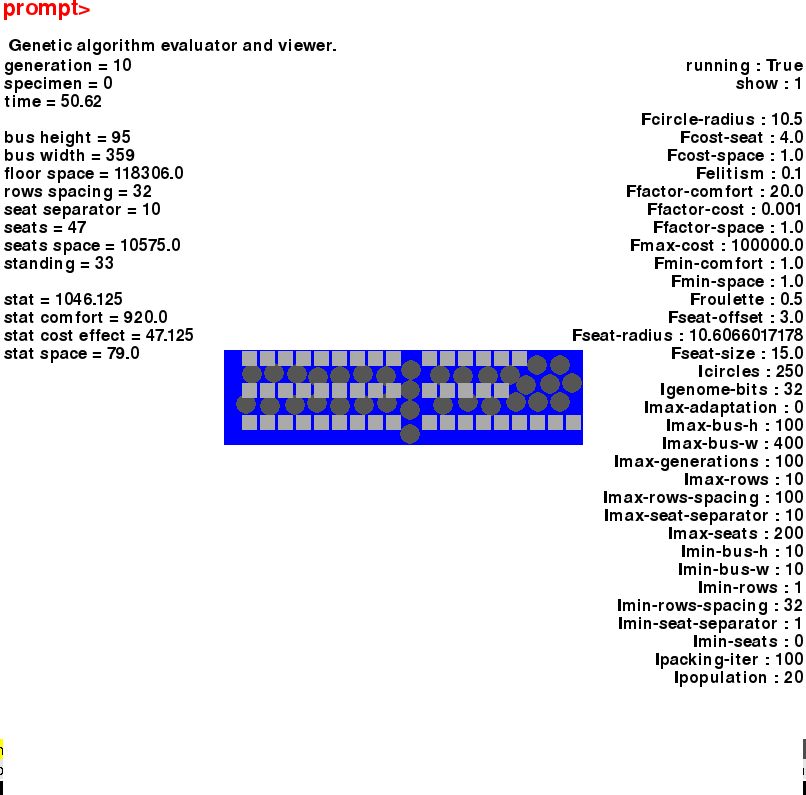
\includegraphics{app-prot2.png}
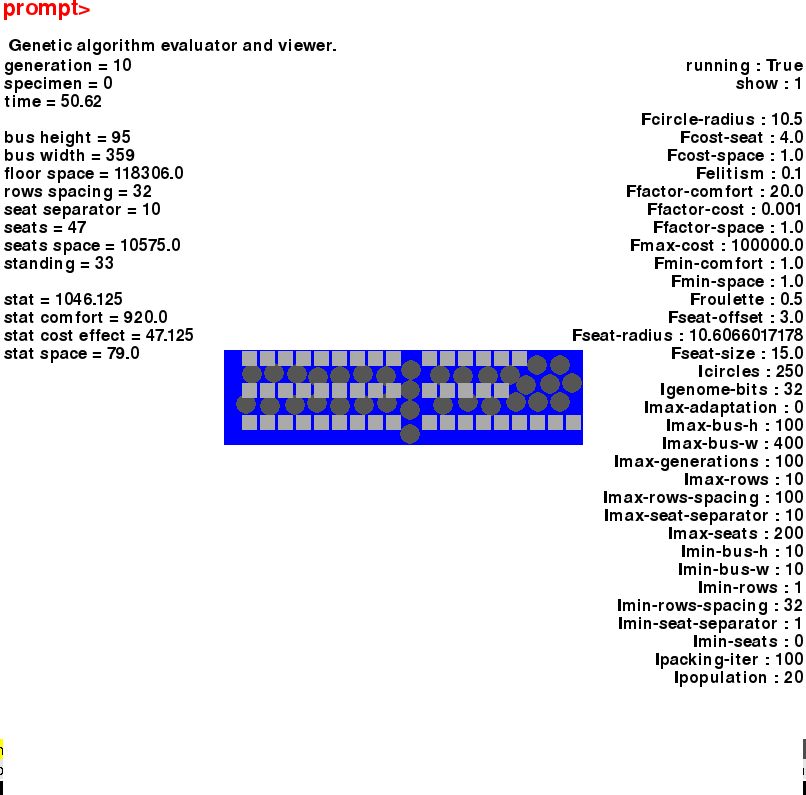
\includepdf{app-prot2.pdf}
%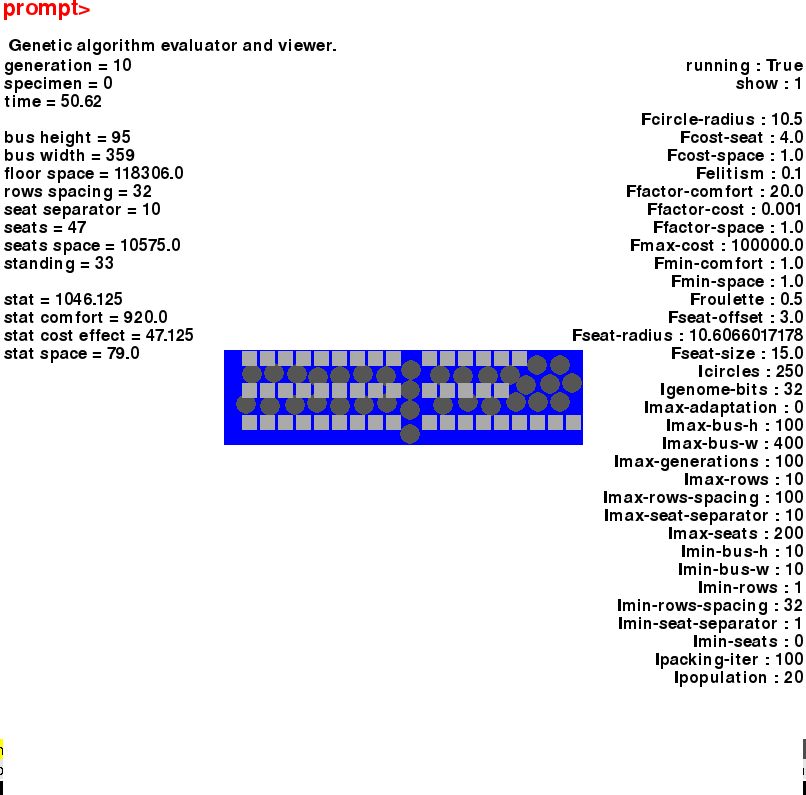
\includepdf[nup=2x2]{app-prot2.pdf}

\chapter{Specyfikacja implementacyjna}
\section{Narzędzia}
Program został zaimplementowany w języku \textbf{Python 2.5}, przy wykorzystaniu biblioteki \textbf{PyGame} wersja \textbf{1.7.1}. Program wykorzystuje moduł \textbf{eztext}, który implementuje prostą linię komend.
Dokumentacja jest generowana za pomocą \texttt{\textit{LaTeX}.}

\section{Pliki i Klasy}
\begin{tabular}{| l || l | p{6cm} |}
\hline
Klasa & Plik & Opis\\
\hline
\hline
- & run.sh  & startuje program\\
\hline
* & src/eztext.py & Moduł (zewnętrzny) implementujący prostą linię komend w PyGame. \\
\hline
- & src/Util.py & Zawiera funkcje pomocnicze.\\
\hline
- & src/Main.py & Punkt wejściowy. Znajduje się tu również główna pętla programu. \\
\hline
Breeder & src/Genetic.py & Klasa implemenująca tworzenie nowej populacji na podstawie starej.\\
\hline
GenerationEvaluator & src/Genetic.py & Klasa wspomagająca wybieranie osobników z generacji.\\
\hline
Generation & src/Genetic.py & Klasa reprezentująca generację osobników.\\
\hline
Config & src/Config.py & Służy do konfiguracji symulacji i parametrów programu.\\
\hline
Specimen & src/Objects.py & Reprezentuje pojedynczego osobnika.\\
\hline
Seat & src/Objects.py & Reprezentuje pojedynczy fotel zawarty w osobniku.\\
\hline
Circle & src/Objects.py & Reprezentuje pojedynczego pasażera.\\
\hline
Overlay & src/Overlay.py & Wyświetla interfejs użytkownika.\\
\hline
\end{tabular}

\section{Opis implementacji algorytmu genetycznego}
\subsection{Kodowanie}
Wszystkie cechy osobników są określone przez liczby całkowite. Są one konwertowane do reprezentacji bitowej ( o długości określonej parametrem Igenome-bits ) za pomocą funkcji Util.int2bin(). Po wykonaniu operacji krzyżowania i mutacji wartości są konwertowane z powrotem to liczb całkowitych za pomocą funkcji Util.bin2int().

\subsection{Krzyżowanie i mutacja}
Łączenie osobników przypomina ``suwak'', który raz bierze wartość od jednego osobnika a raz od drugiego ( Breeder.\_crossover() ). Przed wykonaniem krzyżowania, wszystkie cechy są konwertowane do reprezentacji binarnej i łączone w jeden długi ciąg. Mutacja jest wykonywana na losowych osobnikach przez funkcję Breeder.\_mutate().

\subsection{Określanie przystosowania}
Funkcja określająca przystosowanie ( process\_specimen() w module Genetic ) bierze pod uwagę 3 parametry: komfort ( liczba siedzeń ), koszt ( przesteń zajmowana przez siedzeń i wolna przestrzeń ), oraz całkowita liczba pasażerów w autobusie. Ponadto program bierze pod uwagę wagi poszczególnych parametrów ( Ffactor-comfort, Ffactor-cost, Ffactor-capacity).
Liczba pasażerów jest określana przy pomocy funkcji implementującej algorytm Circle Packing ( Util.pack() )

\subsection{Selekcja}
Selekcja osobników do nowego tworzenia nowego pokolenia odbywa się za pomocą koła ruletki ( GenerationEvaluator.roulette() ). Osobniki o większym przystosowaniu mają większą szansę zostać wybrane przez koło ruletki.
\subsection{Elityzm}
Osobniki, które zostały określone jako najlepsze są przekopiowywane do nowej populacji ( GenerationEvaluator.get\_elite() ).

\end{document}
